% !TEX TS-program = Xelatex
% !TEX encoding = UTF-8 Unicode

\documentclass[UTF8,size=9.5]{ctexart}
\usepackage{amsmath}
\usepackage{dsfont}
\usepackage[table]{xcolor}
\usepackage[bottom]{footmisc}
\usepackage{graphicx}
\usepackage{hyperref}
\usepackage{figsize}
\usepackage{standalone}
\usepackage[separate-uncertainty = true,tight-spacing=true,round-minimum=0.00000000001]{siunitx}
\usepackage{tabu}
\usepackage{wasysym}
\usepackage{geometry}
\geometry{left=0.7in,right=0.7in,bottom=0.7in,top=0.7in}

\title{计算物理学作业3}
\author{朱寅杰 1600017721}
\date{}
\begin{document}
\maketitle
\setcounter{section}{3}
\subsection{Householder与 Givens在 QR分解中的比较}
首先我使用代码实现了这两个算法,源文件分别是\href{./Householder.py}{Householder.py}和\href{./Givens.py}{Givens.py}。

如果使用Householder反射法来对一个$N\times N$方阵进行QR分解,总共需要乘$(N-1)$次反射矩阵。在第$k+1$次反射时,需要算两次一个长度为$N-k$的矢量的模长(每次计算量为$2N-2k$),并作一次归一化($N-k$次除法)。之后的反射,需要对$(N-k-1)^2$个元素进行操作,每个元素算一次点乘和一次旋转,同时把计算$Q$和$R$的工作都算上,要10次计算(可以从我的代码里数出来)。所以总共需要的领头阶计算次数就是$10N^2-20Nk+10k^2$。对$k$求和,得到总的计算次数的领头阶数是$5/3N^3$。

如果使用Givens转动的话,总共有$N(N-1)/2$个下三角元要被归零,每个元$a_{ij}$要被归零,就需要对原来矩阵的两列作Givens转动。每次转动,需要对$N$个矩阵元进行操作,每个矩阵元是三次计算(两次乘法、一次加减法)。同时计算$Q$和$R$,那归零一个$a_{ij}$就需要$12N$次基本计算,于是总的计算次数(领头阶)约为$6N^3$。(另外,在我的代码中,归零$a_{ij}$的顺序是一列一列从左往右来的。如果不按照这个顺序,而按照其他的归零顺序(比如沿着一条条对角线跑),在对$Q$作转动的时候可能可以遇到更多的零元从而减少计算量。但是花费的时间大概也就和原来的算法差一个常数倍数吧。刘川老师有云:为了一个常数倍数的复杂度差别去搞优化是不太值得的,优化的精力要花在算法卡脖子的关键环节上。输出$Q$的操作本不应是算法中很重要的一环,在实际的$QR$迭代中往往都不需要这个过程而是直接乘到矩阵上,所以我也就不去挖空心思搞了。)

对代码进行实际测验,Householder跑$N=6,12,18$跑10000次分别用时1.36s、6.38s、18.5s,Givens跑$N=6,12,18$跑10000次分别用时约1.02s、7.59s、24.6s。分别约摸是$N^{2.4}$和$N^{2.9}$。后者的增长率基本符合预期,而前者的增长率(以及两者运算时间绝对大小的比较)和预期的差距还是蛮大的,一方面和机器的优化等因素有关,另一方面不同的运算的时间也是不一样的,其他如内存存取的时间也没有细细考虑在内。还是请教一个信科的同学让他帮忙估计一下比较靠谱啊。
\subsection{幂次法求矩阵最大模的本征值和本征矢}
对于带有周期性边界条件的微分方程组
\[\ddot{x_{i}}(t)=x_{i-1}(t)+x_{i+1}(t)-2x_{i}(t),x_{i+N}(t)=x_{i}(t),i=1,2,...,N\]
我们求出其(作为解的基底的)简正模式$x_i(t)=x_i\exp(-\mathrm{i}\omega t)$,其中$x_i\in \mathds{C}$,则有
\[-x_{i-1}+2x_i-x_{i+1}=\omega^2 x_i,i=1,2,...,N\]
于是对$x_i$与$\omega$的求解就化为了对一个三对角矩阵$(A_{ij})$的特征值与特征向量的求解,其中$A_{ij}$的具体形式为
\[A_{ij}=2\delta_{ij}-\delta_{(i+1)\bmod N,j}-\delta_{(i-1)\bmod N,j},\enspace i,j=1,2,...,N\]

我们接下来使用Power iteration的办法求解其最大的特征值与特征向量。Power iteration具体是说,对于任意一个可对角化且本征值(的模)非简并的系统$A$,设其本征值(按模长排列)为$\lambda_1>\lambda_2>...$,对应的本征矢量构成一组正交归一的基矢${v_1,v_2,....}$。现在在空间中任取一个单位矢量$a_0=\sum q_iv_i$,其中$q_i\in\mathds{C}$,则有$Aa_0=\sum \lambda_iq_iv_i$。现在我们构造一个迭代:
\[a_0=\sum q_iv_i,a_{i+1}=\frac{Aa_i}{\bigl\lvert Aa_i\bigr\rvert},i=0,1,2,...\]
容易知道
\[a_n=\frac{\sum \lambda_i^n q_i v_i}{\bigl\lvert\sum \lambda_i^n q_i v_i\bigr\rvert}=\bigl(\frac{\lambda_1}{\lvert\lambda_1\rvert}\bigr)^n\frac{q_1v_1+\sum\limits_{i=2}(\lambda_i/\lambda_1)^nq_iv_i}{\Bigl\lvert q_1v_1+\sum\limits_{i=2}(\lambda_i/\lambda_1)^nq_iv_i\Bigr\rvert}\]
由于$\lvert\lambda_1\rvert>\lvert\lambda_2\rvert>...$,因此当$n\rightarrow\infty$时,$a_n$中除了$v_1$上分量外,其他$v_2,v_3,...$上的分量均以指数速度趋于零。故而有
\[\lim\limits_{n\rightarrow\infty}a_n=\lim\limits_{n\rightarrow\infty}[\bigl(\frac{\lambda_1}{\lvert\lambda_1\rvert}\bigr)^n\frac{q_1}{\lvert q_1\rvert}v_1)]\]
忽视掉那个相位因子,我们可以说$a_{\infty}=\lim\limits_{n\rightarrow\infty}a_n=v_1$,因此我们从任意的矢量开始迭代,最终都能收敛到本征矢$v_1$(最多相差一个$U(1)$)。再计算$a_\infty^\dag A a_\infty=v_1^\dag A v_1=\lambda_1$,我们获得了系统最大的本征值。

具体到题中这个一维环形原子链的例子,用上面的迭代算法进行计算(源代码在\href{./power_iteration.py}{power\_iteration.py}),得到的最大本征值为\num{4}(双精度范围内为整数),对应的单位本征矢量为[0.3162277660168382, -0.3162277660168381, 0.316227766016838, -0.3162277660168379, 0.3162277660168378, -0.3162277660168377, 0.3162277660168377, -0.31622776601683783, 0.31622776601683805, -0.31622776601683816],即近似为$[1,-1,1,-1,1,-1,1,-1,1,-1]/\sqrt{10}$。
\subsection{关联函数的拟合与数据分析}
这道题的所有源代码见\href{./cor.py}{cor.py}。首先要对数据进行预处理(题目中叫做“对称化”)。预处理之后我们获得了函数$C(t),t=0,1,...,32$在200次测量下的行为$C_i(t),i=0,...,199$。我们首先通过样本平均估计$C(t)$的中心值,并通过样本方差的平方根来估计每个时间片上$C(t)$的误差。从$t=0$到$t=32$各点的百分误差分别为:
\begin{center}
\begin{tabu} to\linewidth {X[c,-10]|X[c]X[c]X[c]X[c]X[c]X[c]X[c]X[c]X[c]}
\hline
$t$&0	&1	&2	&3	&4	&5	&6	&7	&8\\
\hline
百分误差&1.58 	&2.36 	&5.64 	&8.30 	&10.37 	&11.91 	&13.12 	&14.07 	&14.85\\
\hline\hline
$t$&9	&10	&11	&12	&13	&14	&15	&16	&17\\
\hline
百分误差&15.20 	&15.39 	&16.01 	&16.56 	&17.15 	&17.79 	&18.29 	&18.88 	&19.43\\
\hline\hline
$t$&18	&19	&20	&21	&22	&23	&24	&25	&26\\
\hline
百分误差&19.87 	&20.10 	&20.30 	&20.57 	&21.04 	&21.56 	&22.09 	&22.42 	&22.67\\
\hline\hline
$t$&27	&28	&29	&30	&31	&32	&	&	&\\
\hline
百分误差&22.90 	&23.17 	&23.48 	&23.71 	&24.17 	&24.48 	&	&	&\\
\hline
\end{tabu}\end{center}
然后是分别通过两种方法算有效质量。通过直接做比值的办法,取$m_{eff}=\log\frac{C(t)}{C(t+1)}$,按每自由度卡方最优拟合出来的平台位置在[24,27]处,自由度为3,$\chi^2/d.o.f=0.1093$,查表得相应的$p$值为0.0453。拟合出的粒子质量为\num{1.157124(105)}(误差按1$\sigma$计,是从输出结果里面截取数据然后拿计算器解的二次方程)。

通过更加精确的$m_eff=\cosh^{-1}(\frac{C(t+1)+C(t-1)}{2C(t)})$的办法,按每自由度卡方最优拟合出来的平台位置在[25,29]处,自由度数为4,$\chi^2/d.o.f=0.08979$,查表得相应的$p$值为0.0143。拟合出的粒子质量为\num{1.157100(109)}(误差也是敲计算器解的方程)

然后算的是两个相关系数咯。$\rho_{3,4}=\num{0.95706(631)}$,$\rho_{3,5}=\num{0.90101(1621)}$,

\begin{figure}
  \centering
  \SetFigLayout{2}{1}
  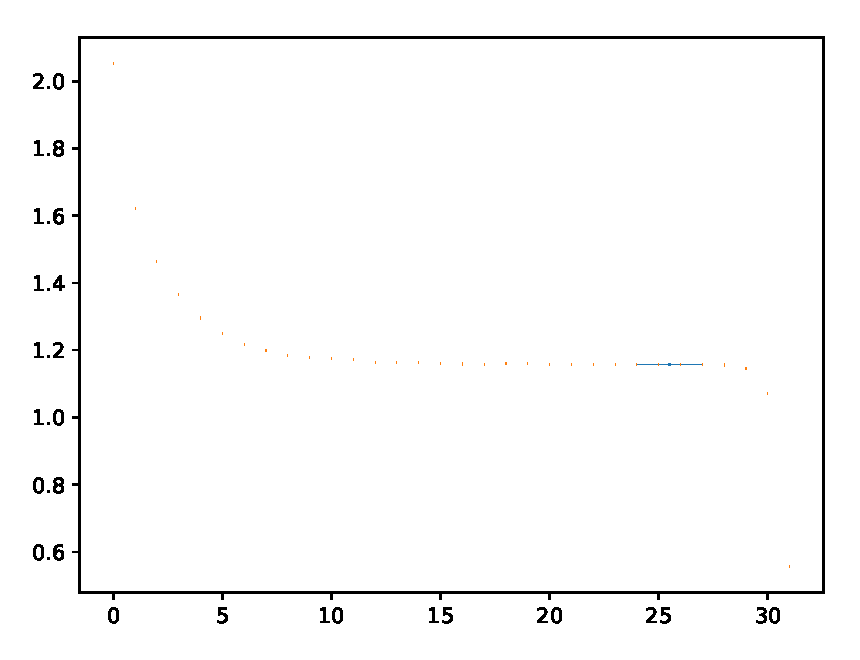
\includegraphics[width=0.8\linewidth]{ratio.eps}
  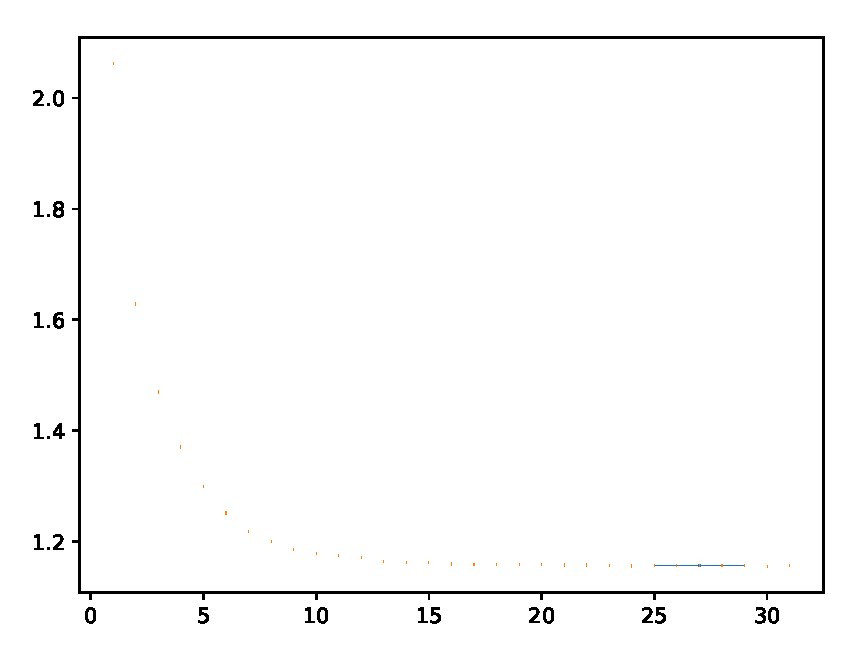
\includegraphics[width=0.8\linewidth]{acosh.eps}
  \caption{横轴是$t$,纵轴是$m_{eff}$。如果你发现什么都看不见的话,那就对了,因为error实在是太小了,以至于我都不能把数据点画大,不然就都盖住什么都看不见了。上图是用比值法算的$m_{eff}$及其误差,下图是用arccosh法算的。卡方拟合的区间和error bar也画在图里了(不对,似乎error bar也被盖住了。不管它,反正我数字算出来了)。如果你看不见的话,zoom in,zoom in,再zoom in(我是矢量图我无所畏惧.eps)。如果还是嫌error bar看不清的话,就跑一下程序\href{./cor.py}{cor.py},看一看输出结果吧。各个点的位置和误差都在上面了。}
\end{figure}
\end{document}


